% v2-acmtog-sample.tex, dated March 7 2012
% This is a sample file for ACM Transactions on Graphics
%
% Compilation using 'acmtog.cls' - version 1.2 (March 2012), Aptara Inc.
% (c) 2010 Association for Computing Machinery (ACM)
%
% Questions/Suggestions/Feedback should be addressed to => "acmtexsupport@aptaracorp.com".
% Users can also go through the FAQs available on the journal's submission webpage.
%
% Steps to compile: latex, bibtex, latex latex
%
% For tracking purposes => this is v1.2 - March 2012
\documentclass{acmtog} % V1.2
\usepackage{float}
\usepackage{graphicx}
\usepackage{subfigure}
\usepackage{algorithm2e}
%\acmVolume{VV}
%\acmNumber{N}
%\acmYear{YYYY}
%\acmMonth{Month}
%\acmArticleNum{XXX}
%\acmdoi{10.1145/XXXXXXX.YYYYYYY}

\acmVolume{0}
\acmNumber{0}
\acmYear{2019}
\acmMonth{January}
\acmArticleNum{0}
\acmdoi{10.1145/0.0}

\begin{document}

\markboth{H.T. Tang}{Learning Very Sparse Convolution Under a Pseudo-Tree Constraint}

\title{Learning Very Sparse Convolution Under a Pseudo-Tree Constraint} % title

\author{Hao-Tian Tang
\affil{Shanghai Jiaotong University}
}
% NOTE! Affiliations placed here should be for the institution where the
%       BULK of the research was done. If the author has gone to a new
%       institution, before publication, the (above) affiliation should NOT be changed.
%       The authors 'current' address may be given in the "Author's addresses:" block (below).
%       So for example, Mr. Fogarty, the bulk of the research was done at UIUC, and he is
%       currently affiliated with NASA.


\terms{Convolution, Compression}

\keywords{Sparse convolution, deep neural networks, network compression}



\maketitle



\begin{abstract}
The convolution operation is very common in today's artificial intelligence tasks. Though the convolution operation takes advantage of parameter sharing and reduces the number of parameters by an order of magnitude comparing with the fully-connected matrix multiplication operation, there are still large redundancy in the convolution operation.

Inspired by the intuition of group convolution and the sparsity of the tree structure, we propose a novel idea in this paper which reduces the number of parameters involved in a convolution operation, in the circumstance of image classification with deep neural networks. We propose to group some feature maps in the input/output of a convolution layer, and find a maximum cardinality matching between the input nodes and output nodes of a convolution operation. Additionally, we constrain the final output network to be tree-structured to further reduce the number of parameters.

In terms of neural network pruning, our method gives a structured pruning approach, which achieves high compression rate comparable with weight-level pruning (which is not structured). In our experiments on CIFAR-10, we are capable of reduce the number of parameters in the VGG16 network by 24x, the number of parameters in the ResNet164 by 2.5x, and DenseNet by 3x, with small accuracy loss.
\end{abstract}

\section{Introduction}

The neural networks are very computation intensive. Despite the fact of convolution operations, the most common operation in today's deep neural networks, utilizes the property of parameter-sharing and thus reduce the number of parameters required to output the same feature map with matrix multiplication by an order of magnitude, it is still accepted by most people that the convolution operation is highly redundant.

If we examine the convolution operation as a graph like what is done in figure \ref{fig:conv}, we can very easily find out that the convolution operation can be viewed as a fully-connected bipartite graph. However, to make the graph connected, it is not necessary to maintain a maximal-sized bipartite graph. As is illustrated in figure \ref{fig:tree}, the tree-structured neural network in which one feature map is calculated through only one predecessor is sufficient to maintain the connectiveness of the whole computation graph. 

Of course, the tree-structured neural network is seriously constrained in computational capability, as it's similar to a depthwise convolution operation without the pointwise convolution. With the presentation of a pointwise convolution, the computational capability of a depthwise convolution is limited, not to mention the version without it. So we don't consider to transform a traditional convolution operation to a tree-structured convolution, which will make it too difficult for the network to retain the computation capability.

\begin{figure}
\centering
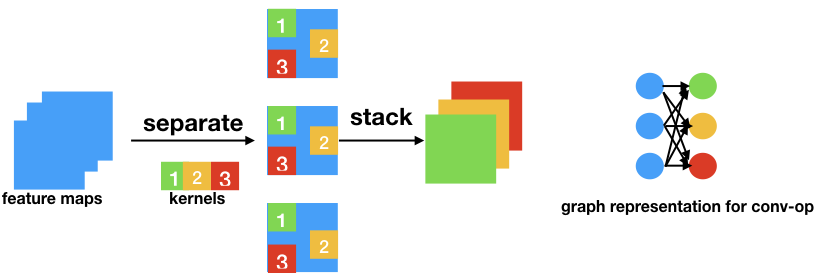
\includegraphics[width=1\linewidth]{assets/conv.png}
\caption{The graph representation of a convolution operation. Each channel of the input and output feature map is viewed as a node in a graph, and the vertices between two nodes indicate that the right-hand-side node is calculated with the left-hand-side node.}
\label{fig:conv}
\end{figure}

\begin{figure}
\centering
\subfigure{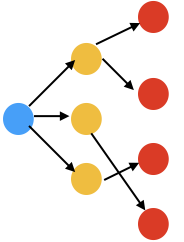
\includegraphics[width=0.3\linewidth]{assets/tree-network.png}}
\subfigure{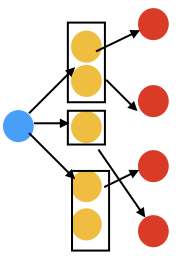
\includegraphics[width=0.3\linewidth]{assets/pseduo-tree.png}}
\caption{Left: The minimal connection form: A tree-structured neural network. Right: Restoring some computation capability by grouping some nodes in a tree network together.}
\label{fig:tree}
\end{figure}

However, we can group some nodes in a layer together in the original computation graph as what is done in the right hand side part of \ref{fig:tree}. After the grouping, we allow the connection between two groups to be fully connected (i.e. for a feature map in each group, it is calculated with all the feature maps in its predecessor group). In order to still remove a large number of parameters in the neural network, we force each group to be calculated from only one predecessor group. Such constraint is called the \textbf{pseudo-tree constraint} in this paper, because the computation graph cannot be viewed as a tree in the level of feature maps, but it is indeed a tree in the level of feature-map group. In this case, the parameter reduction ratio of each convolution operation can be proved to be \textbf{at least the number of groups}. The term \emph{at least} comes because some nodes can be cutoff from the computation graph because of the tree constraint. For example, if a layer $l+1$ has $N$ nodes and its exact predecessor layer $l$ has $N+k$ nodes, then at least $k$ nodes in layer $l$ is naturally disconnected from the graph. This effect can also be viewed as automatic and parameter-free channel pruning.

Notice that we just group nodes together sequentially (The channels that are contiguous in memory are grouped together) in figure \ref{fig:tree}, but it is not a constraint in real implementations. Actually, grouping sequentially is just what \emph{group convolution} does. In our proposed pseudo-tree constrained convolution scheme, it is allowed to form the groups arbitrarily, so that our framework is very suitable for the task of pruning a pretrained neural network. Obviously, under such scene, it is not reasonable to impose a strong prior of sequential grouping.

As we will point out later, by utilizing the sparsity of our proposed pseudo-tree constrained structure and the automatic channel pruning effect, we can compress some state-of-the-art neural networks including the VGG networks, the ResNets and the DenseNets by very impressive ratios. To point out, we achieve much higher compression rate (2.5x V.S 1.4x) comparing with the network slimming method proposed by \cite{networkslimming}, while retain the same accuracy to this channel-level pruning algorithm. For the VGG network and DenseNet, our proposed method can easily achieve very high compression ratio. For example, we prove that the last several convolution layers in VGG can be pruned by a factor of 120x, without any loss of accuracy on CIFAR-10. Such ratio exceeds the result in many network pruning works by an order of magnitude. Unfortunately, we failed to figure out the way to solve the accuracy drop, but we believe the setting of group numbers might be a reason, and we don't have enough time to tune these parameters.
\section{Related Work}
Due to the popularity of the convolution operation, there are countless approaches to optimize it. Some focus on the mathematics behind convolution itself, others, like this paper, focus on optimizing the performance of the convolution operation in the concept of a neural network. Also, there're some works focused on tree-structured network (where the basic node in the computation graph might be a basic block like residual block). All of these works are related to this paper and will be introduced briefly.
\subsection{Efficient Convolution Operation}
There are many attempts to reduce the computational cost and memory footprint of the convolution operation. Some methods are equivalent to the original convolution operation, but saves computation through transformations and inverse transformations. For example, the FFT-based method proposed by \cite{FFT}, and the Winograd convolution algorithm proposed by \cite{winograd}.

There are also other works of \emph{loss} convolution approximation. For example, previous works use SVD method to approximate the convolution operation, while \cite{SVD} goes beyond SVD, and uses higher order approximation and filter clustering to reduce the memory consumption and computational requirement of the convolution operation. 
\subsection{Deep Neural Network Compression}
Some papers also focus on the compression of deep neural networks. There are coarse-grained DNN pruning and fine-grained DNN pruning algorithms.

For the coarse-grained DNN pruning algorithms, the common objective is to prune some channels which are considered to be less important. For example, \cite{networkslimming} considers to utilize the coefficient for the batchnorm operation as an indicator of the importance of each channel, and prune channels with small coefficients to compress the model. \cite{pruneverydeep} uses LASSO regression to select the channels. Selecting the channels directly based on the norm of the channels is also possible in \cite{amc}. To point out, \cite{amc} also utilizes the deep reinforcement learning method to automatically determine the sparsity ratio of each layer.

For the fine-grained DNN pruning, the main concern is usually pruning the redundant weights. For example, \cite{hansongnips15} proposes to iteratively prune and retrain the deep neural networks, and achieves very high compression rates on multiple state-of-the-art neural networks. Following this work, \cite{hansongICLR2016} also puts forward trained quantization and Huffman coding to further reduce the memory cost of DNNs. However, the fine-grained pruning algorithms are always \textbf{unstructured}. To achieve real speedup, special hardware such as the EIE \cite{EIE} must be consulted.
\subsection{Tree-Structured Neural Networks}
Because of the sparsity of tree-structured connections, a lot of works focus on tree-structured neural networks. For example, \cite{GNAS} searches for tree-like structures for multi-attribute learning in facial attributes, and achieves state-of-the-art results with far less parameters than previous methods. \cite{caihan} is also a paper in neural architecture search, a very efficient tree-structured basic block is introduced in this paper.
\section{Proposed Method}
\begin{algorithm}
\SetAlgoLined
\KwData{Convolutional Filters $K_1, K_2, ..., K_N$ in the network. Layer groupings $G_1, G_2, ..., G_N$.}
\KwResult{A set of masks $M_1, M_2, ... , M_N$ for the filters.}
Initialize $M_i = 0 (\forall{i})$.\\
\For{i=N; i$\geq$0; i--}{
	Initialize A $g_i\times g_{i+1}$ table $T$, where $g_i$ is the number of channels in layer i.\\
	\For{j = 0; j $<$ $g_i$; j++}{
		Mask all $K_i$ parameters except for those for $G_j$.\\
		Train the neural network for 100 iterations.\\
		Update row $j$ of the $T$. $T_{jk}$ is the average descendent class accuracy of the $k^{th}$ group in layer $l+1$.\\
	}
	Selection = argmax($T$, axis=0).\\
	Reconnect layer $i$ according to the Selection. Update $M_i$ accordingly.\\
	Update the descendent class information for layer $i$.\\
	\If{$G_i$ has no descendent class}{
		Remove $G_i$ from computation graph.
	}
}

\caption{Sparse Convolution Algorithm.}
\label{alg:VSConv}
\end{algorithm}

We have already introduced the intuition of pseudo-tree constraint in previous sections. We will mainly introduce in this section how to determine the predecessor of each feature-map group (which is a node in our computational graph), and also how to generate the groupings. Our connection selection algorithm is inspired by \cite{GNAS}. The major difference is that they use this idea mainly to search for connections between basic blocks, which is common in the scene of NAS. However, our focus is to search for connections between feature maps, within one convolution operation.

The pipeline of our algorithm can be summarized in algorithm \ref{alg:VSConv}. The algorithm sketch is too simple, and it is actually implemented in about 500 lines of Python code. For details, please refer to the github repository related to this paper.

\subsection{Problem Formulation}
We have illustrated our problem formulation through figure \ref{fig:tree} informally in the introduction section. To make it more formal, we define the problem as follows:

For a neural network $\mathcal{N}$ with $N$ layers, denote all its feature maps as $F_1, F_2, ..., F_N$. Each feature map group $F_i = [f_1^{(i)}, ..., f_C^{(i)}]$, if it has $C$ channel groups. Also denote all the convolution kernels as $K_1, ..., K_{N-1}$. Notice that the fully connected layer is also viewed as $1\times1$ convolution.  We have $F_{i+1} = Conv(K_i, F_i)$. Our target is to zero away most parameters in $K_i$.

For $f_k^{(i+1)}(\forall k)$, we have $f_k^{(i+1)} = h(f_1^{(i)}, f_2^{(i)}, ..., f_C^{(i)}$), where $h$ is a linear combination, defined as part of the convolution operation. The coefficients of $f_i^{(k)}$ is related to the coefficients of $K_i$. To be specific, we want only one coefficient of $f_k^{(i)}$ to be nonzero, and others are all zero (pseudo-tree constraint). This can be formulated as introducing a mask $M_i$ to $K_i$, in which the second dimension of $K_i$ is only non-zero corresponding to one feature map group of $F_i$.

As long as the pseudo-tree constraint is satisfied, we want the overall accuracy of classification to be maximized.
\subsection{Connection Selection for the Whole Network}
We have already formulated the problem of connection selection in kernel coefficients $K_i$ as determining the kernel mask $M_i$. Potentially, we need to decide $\{M_1, M_2, ..., M_{n-1}\}$ simultaneously. For each $M_i$, the potential choices of zeroing is the number of groups $g_i$ for the corresponding layer. So the total complexity will be $O(g^n)$, where $g$ is the maximal number of groups. The computation burden is not affordable, and we need to approximate the process of mask learning. 

We introduce the Markovness assumption in the mask learning process. We assume that the selection of $M_i$ is independent of $M_j, j\neq i$. We can understand this assumption in another way. Originally, we have $F_{i+1} = Conv(K_i, F_i)$. Now, we use $\hat{F}_{i+1} = Conv(K_i\circ M_i, F_i)$. If the approximation $\hat{F}_{i+1}$ is close enough to original feature map $F_i$, then the Markovness assumption should be very reliable, because introducing $M_i$ will almost not change the output of each convolution operation (that means, for each $i$, having $M_i$ or not doesn't influence the output, so the $M_j$ doesn't influence $M_i$, if $j\neq i$), thus, $M_i$ can be dealt with separately. 

Although we don't explicitly force our masked convolutional filters to approximate the original feature map (by exerting some regression loss), such formulation will help justify our Markovness assumption, which easily simplify the computational cost of our proposed method to $O(gn)$, where the oracle operation is to determine a group-group connection in one convolution filter.

Here comes another problem. Now that we have decided to determine $M_i(i=1,2,...,N)$ independently, the order of determining these masks matters. In this paper, we follow the conventions in \cite{GNAS} by selecting the masks $M_i$ reversely, from $M_N, M_{N-1}, ...$ to $M_1$. Furthermore, we assure $M_{k+1}, M_{k+2}, ..., M_{N}$ already constrains convolution operations starting from layer $k+1$ to a pseudo-tree, when we are trying to determine $M_k$. The intuition is illustrated in figure \ref{fig:method1}. We will illustrate in next section that such \textbf{reverse order} is necessary for the single layer connection selection.

\begin{figure}
\centering
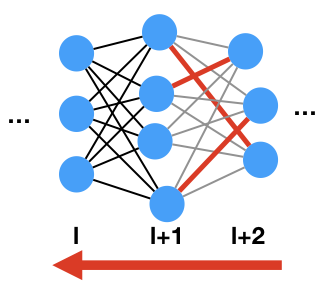
\includegraphics[width=0.5\linewidth]{assets/method1.png}
\caption{Illustration of the idea of reverse mask selection. When we are going to determine the $M_l$, we assume the connection between layer $l+1$ and layer $l+2$ has already been determined, and the structure after layer $l+2$ has already been a forest. The nodes in this graph is also defined as feature map groups.}
\label{fig:method1}
\end{figure}

\subsection{Single Layer Connection Selection}

\begin{figure}
\centering
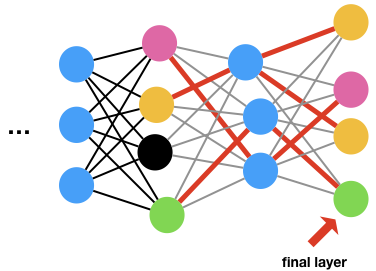
\includegraphics[width=0.5\linewidth]{assets/decendent.png}
\caption{Illustration of the idea of descendent classes. Let's focus on the second leftmost column in this computation graph. Each final class has a color. For each node in the left column, if their a path to a particular final class, then this node will share the color with the final class, and the final class is called its \textbf{descendent class}.}
\label{fig:descendent}
\end{figure}

We have decided to determine masks $M_i$ in the order $M_N, M_{N-1}, ..., M_1$. In this section, we will introduce the algorithm of determining single $M_i$. To determine $M_i$, we believe the most important criteria is the accuracy. Obviously, the global accuracy (i.e. the average accuracy of all classes) is indiscriminative and not helpful for our task of connection selection within a layer, because this statistic remains the same for all connections. So we propose to use a kind of \textbf{local accuracy} (this idea is similar to GNAS\cite{GNAS}).

Recall that when we are determining $M_l$, the connections from layer $l+1$ to layer $N$ is already a pseudo-tree, or a forest structure. In this case, we will see a situation like what is shown in figure \ref{fig:descendent}. The leftmost layer can be viewed as layer $l$, and the second leftmost layer can be viewed as layer $l+1$. In this graph, we have visually defined the descendent classes of each node in layer $l+1$, and the formal definition is given in the caption. Having the information of \textbf{descendent classes}, we can always calculate a scalar for each node in layer $l+1$, which is the average descendent class accuracy for this given node. As we move on to layer $l, l-1, ..., 1$, this scalar will be used to select connection.

\begin{figure}
\centering
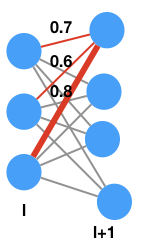
\includegraphics[width=0.3\linewidth]{assets/method2.png}
\caption{Illustration of connection selection. We use the node 1 in layer $l+1$ as an example. We will try to connect node 1,2,3 of layer $l$ to it respectively. After a connection is made, we can get a weight on the connection, which is the \textbf{average descendent class accuracy} define previously. Obviously, the connection to node 3 of layer $l$ gives the highest accuracy, so this connection is selected (in bold).}
\label{fig:selection1}
\end{figure}

\begin{table*}[t]
\tabcolsep22pt
\tbl{Summary of the performance of different models after using the proposed algorithm.
}{%
\begin{tabular}{@{}ccccc@{}}\hline
Network &{Parameters(before)} &{Parameters(after)} & {Accuracy(before)} & {Accuracy(after)} \\
\hline
VGG16 & 20051530 & 825160 & 92.80 & 89.50 \\
ResNet164 & 1727645 & 670237 & 93.45 & 92.90 \\
DenseNet40 & 1078057 & 350572 & 93.86 & 90.00\\
\hline
\end{tabular}}
\label{tab:experiments}
\end{table*}

\begin{table}
\tabcolsep22pt
\tbl{Summary of the compression ratio. Compared with network slimming.
}{%
\begin{tabular}{@{}ccc@{}}\hline
Network &{Compression Ratio} & {Network Slimming} \\
\hline
VGG16 & 24.30 & 8.28 \\
ResNet164 & 2.58  & 1.41\\
DenseNet40 & 3.08 & 2.20\\
\hline
\end{tabular}}
\label{tab:compression}
\end{table}


To be specific, let's consider the connections between layer $l$ and layer $l+1$. For simplicity, we just illustrate how to select connection for one node in layer $l+1$, the whole process is just to iterate over all nodes in layer $l+1$. We consider the node 1 of layer $l+1$ in figure \ref{fig:selection1}. As can be seen from the figure and caption, the connection with node 3 of layer $l$ leads to the best descendent class average accuracy, which is 0.8, so this selection tends to be selected by our algorithm.

Of course, this process can be quite slow. The three connections in red in figure \ref{fig:selection1} cannot be evaluated in parallel. The reason is that the connection before layer $l$ is still fully connected. If the three connections are evaluated in parallel, we can get only one average descendent class accuracy for the connection, and we don't know what the accuracy means. Hence, suppose the number of groups in layer $l$ is $g_l$, number of groups in layer $l+1$ is $g_{l+1}$, the connections we have to try is $g_l g_{l+1}$. This quadratic complexity is intolerable for deep neural networks such as ResNet164.

The solution is quite simple. We cannot avoid filling in a descendent class accuracy table of size $g_l g_{l+1}$. However, instead of trying to fill in one column at a time (i.e. evaluate the connection from all nodes in layer $l$ to one node in layer $l+1$), we want to determine one row at a time. That is, we can connect one node in layer $l$ to all the nodes in layer $l+1$ simultaneously. Note that this is valid, because the intersection of descendent sets of any two nodes in layer $l+1$ will always be empty (because of the pseudo-tree constraint). By doing so, we successfully make the $g_{l+1}$ term disappear (in parallel computation). The overall complexity of connection search is $O(g_l)$, which is affordable.
\subsection{Dealing with Multi-Branch Networks and Skip Connections}
Basically, the multi-branch neural networks and neural networks with skip connections cannot be pruned to a pseudo-tree structure. However, we can still relax the constraint a little bit to make it possible to use the previous algorithm. Notice that the algorithm is run from backward to forward, so the skip connection will never break the \textbf{descendent class set} of each node, so the criterion is still valid, we can still run the algorithm. Intuitively, the number of paths in multi-branch neural networks is exponential to the number of layers, so it is not possible to prune the multi-branch neural network in the path-level. i.e. It is not possible to consider the impaction on path on the other. However, the good news is that, the number of convolution operations in a multi-branch neural network is limited. Suppose the number of layers is $N$, the largest branch number is $K$, then the number of convolution operations is less than $NK$. So the overall complexity of the previous connection selection algorithm is just enlarged by a constant. For networks like the ResNets who have only two branches, the additional overhead is tolerable.
\section{Experiments}

We conduct our experiments in the setting of image classification. Due to the limitation of computational resources, we chose CIFAR-10 \cite{CIFAR} as our dataset. We implement the standard VGG16 network with batch normalization (with around 20.04M parameters), the standard ResNet164 network (with around 1.71M parameters) and the DenseNet40 network (with around 1.07M parameters) to illustrate the effectiveness of our algorithm in both single-branch and multi-branch networks with skip connections.
\subsection{Dataset}
The CIFAR-10 datasets \cite{CIFAR} consist of natural images with resolution 32$\times$32. There are 50000 images in the training set, we use 90\% of them as our training data and leave the other 10\% for validation. The test dataset contains 10000 images. In training, we use padding, random horizontal flipping, random clipping data augmentation. We remove all the data augmentation in the testing phase.
\subsection{Experiment Results}
We conduct our experiments using three popular neural networks. As can be seen from tables \ref{tab:experiments} and \ref{tab:compression}\footnote{The compression rate becomes much higher than what is mentioned in mid-term presentation because we cut off the nodes who do not have descendent classes from the computation graph.}, the method is able to give very high compression rate, while slightly lose some accuracy. Since the accuracy is measured after finetuning our network, we still have a long way to go before having some impactful results.

To point out, in the experiments, \textbf{the number of groups in each layer} has great impact on the final result. For example, for VGG16, if the number of groups in the last several layers is set to be very large (like 32), the accuracy is not influenced. However, for some critical layers (e.g. layer 7), if the group number is set to be large (say, 8), the accuracy drops dramatically. For all networks, the group number parameter for all layers can be found in our code. We just set first $\frac{1}{4}$ layers to have group number 1, last $\frac{1}{4}$ layers to have group number 4, and others to have group number 2 for ResNets and DenseNets. For the ResNet164, actually we even didn't prune any layer before layer 115, and the compression ratio is already impressive. For the VGG16 network, we set these parameters by hand, the largest group number can be 16 or 32.

For comparison with network slimming, we reproduced this work in PyTorch by ourselves. For VGG and DenseNet, we observed around 0.1\% accuracy improvement in their work, while we observed exactly the same accuracy loss as our method when pruning ResNet164 using their proposed method. We believe our method will have better accuracy performance when the compression rate is lower, but we don't have time to tune our model carefully.

We also illustrate the compression rate of the VGG16 network layer by layer in figure \ref{fig:comp}. As can be seen from the figure, we are able to reduce the number of parameters in some last convolution layers by a factor of more than 100, which is quite astonishing. The 100x compression factor is contributed by both automatic channel pruning (cutting off the nodes which don't have descendent classes) and learned sparse connection. With only learned sparse connection, the compression rate for a layer can hardly exceed 32x. We believe that if the accuracy can be restored, this work will be quite valuable in terms of memory efficiency.

\begin{figure}
\centering
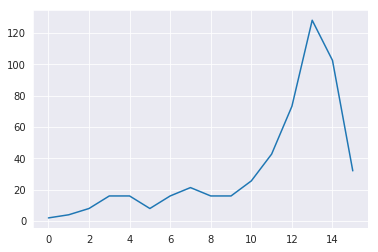
\includegraphics[width=\linewidth]{assets/compression.png}
\caption{The compression rate for the VGG16 network, shown layer by layer. The highest compression rate for a single \textbf{convolution} layer achieves 120x. Note that channel pruning (structured) methods rarely prune a convolutional filter by more than 10x.}
\label{fig:comp}
\end{figure}

\section{Conclusion}
We demonstrate the value of tree-structured constraint in neural network pruning. Although we didn't retain the accuracy of the original neural networks after retraining, we found that some last convolution layers do have a redundancy of around 100x, which is astonishing. We also discovered in experiments that some layers in some network such as VGG are critical because they are very volatile to high compression rate.

There are lots of things not done in this project. For example, it is the current trend that the parameters like \emph{sparsity ratio}, or \emph{number of groups} (in this paper) are not determined by human-beings. The wide use of DDPG agents in design automation \cite{amc} have naturally inspired us to integrate reinforcement learning into this paper. However, channel selection is cheap, while our connection selection is expensive (with 100 iterations of retraining, though only one layer is updated). The usage of RL may not be so obvious under limited computation budget.

Another thing is to implement this algorithm for real hardware. Currently, what we have done is only zero away a large number of weights, instead of \textbf{really make them disappear}. We didn't do anything to \textbf{speedup} computation, either. Naturally, because of the structured pruning property, we expect our algorithm to work pretty well on FPGAs and ASICs, since we have smaller indexing overhead than previous weight-level pruning algorithms. However, whether our method can achieve latency performance comparable with some recent work tailored for target hardware (also using DDPG agents) is questionable. We have to admit that we break some spatial locality in our pruned models, which may make speedup negligible.
% Bibliography
\bibliographystyle{ACM-Reference-Format-Journals}
\bibliography{acmtog-sample-bibfile}
                                % Sample .bib file with references that match those in
                                % the 'Specifications Document (V1.5)' as well containing
                                % 'legacy' bibs and bibs with 'alternate codings'.
                                % Gerry Murray - March 2012

\received{September 2008}{March 2009}

\end{document}
% End of v2-acmtog-sample.tex (March 2012) - Gerry Murray, ACM
